\section{Robustness}
\label{sec:Robustness}
The field measurements showed.
\cite{smolnik_5g_2020} \SI{3}{\metre} corn plants
Therefore, the following section focuses on the influence of the different physical layer parameters on the robustness of the IEEE 802.11ax standard
Wi-Fi transmissions.

A known simulation tool for wireless communication networks is GNU Radio \footnote{https://www.gnuradio.org/}.
GNU Radio is an open-source software development toolkit, which has additional blocks for IEEE 802.11 network simulation,
called gr-ieee802-11 \footnote{https://github.com/bastibl/gr-ieee802-11}. However, the gr-ieee802-11 only
supports the IEEE 802.11a, IEEE 802.11b, IEEE 802.11g and IEEE 802.11p. This means, that the gr-ieee802-11 does not support
the \ac{ER} mode, \ac{DCM} or \ac{STBC}. Therefore, I decided that the GNU Radio is not suitable for my simulation.

\textcite{s_performance_2022} cites ns-3 \footnote{https://www.nsnam.org/docs/models/html/wifi-design.html},
that ns-3 does not implement
any frequency-selective fading effects, such as multipath propagation and shadowing. Therefore, the authors decided to use
the MATLAB WLAN Toolbox, which is standards-compliant and credible.
I also decided to use Matlab because besides \cite{s_performance_2022}, \cite{cao_efficient_2022} and \cite{jin_efficient_2021} have also considered
the MATLAB WLAN Toolbox to be suitable for IEEE 802.11ax simulations.

The MATLAB WLAN Toolbox \footnote{\url{https://de.mathworks.com/products/wlan.html?s_tid=AO_PR_info}} is a add-on to simulate, analyse, and test of wireless LAN communications systems.
The WLAN Toolbox supports a wide range of IEEE 802.11 standards.
Since Release R2019b \footnote{https://de.mathworks.com/help/wlan/release-notes.html}, the WLAN Toolbox supports the Signal Recovery, Packet Extension and Physical Layer abstractions to simulation IEEE 802.11ax networks.

My robustness analysis is based on the WLAN Toolbox example wlan/HESUExample \footnote{https://de.mathworks.com/help/wlan/ug/802-11ax-packet-error-rate-simulation-for-single-user-format.html} to simulate the \ac{PER} of point-to-point IEEE 802.11ax networks for
a specified \ac{SNR} values.

First, I set the IEEE 802.11ax physical layer parameters using the wlanHEConfig object,
where I define the default settings in \autoref{tab:robustnessDefaultSettings}.

\begin{table}
	\centering
	\begin{tabular}{>{\raggedright}p{4.5cm}p{4.5cm}}
		\toprule
		Parameter & Chosen Default Settings \\
		\midrule
		\ac{GI} & \SI{3200}{\nano\second} \\
		\ac{BW} & \SI{20}{\mega\hertz} \\
		Number Spatial Streams & \num{2}\\
		Number Transmit Antenna & \num{2} \\
		\ac{DCM} & disabled \\
		\ac{STBC} & disabled \\
		\ac{HE}-\ac{MCS} & \num{0} \\
		\ac{ER} & disabled \\
		\ac{LDPC} & enabled \\
		\bottomrule
	\end{tabular}
	\caption{Default physical layer settings for the IEEE 802.11ax robustness simulations}
	\label{tab:robustnessDefaultSettings}
\end{table}

Next, I chose a channel model to simulate the channel.
The WLAN Toolbox supports a wide range of channel models, such as wlanTGaxChannel, wlanTGnChannel, wlanTGacChannel, and wlanTGnChannel.
The wlanTGaxChannel model supports \num{6} different channel models for IEEE 802.11ax networks, named TGax-A, TGax-B, TGax-C, TGax-D, TGax-E, and TGax-F,
where the TGax-F channel model is suitable for pseudo-outdoor scenarios \cite{TGAXCHANNEL}.
The TGax channel models were used for Matlab Wlan Toolbox simulations by \cite{s_performance_2022}, \cite{cao_efficient_2022} and \cite{jin_efficient_2021}.

\cite{TGAXCHANNEL} and \cite{omar_survey_2016} list, that IEEE 802.11ax task group has also implemented the channel models UMa and UMi for
outdoor urban scenarios.
However, the WLAN Toolbox does not support these channel models and they are intended for urban scenarios, which

As I want to simulate outdoor scenarios, I chose the TGax-F channel model, which is suitable for pseudo-outdoor scenarios \cite{TGAXCHANNEL}.
The wlanTGaxChannel model supports configuring the \ac{BW}, the number of transmit and receive antennas, which I set equal to the configuration of the wlanHEConfig object.
\cite{freq_plan_24G} and \cite{freq_plan_5G} allow outdoor transmission in the frequency range of \SI{5.725}{\giga\hertz} to \SI{5.825}{\giga\hertz}. Therefore, I set the carrier frequency to \SI{5.6}{\giga\hertz}.
The TGax-F channel sampling rate is set to \SI{20}{\mega\hertz}, which is the nominal sampling rate for the configured \ac{BW} of \SI{20}{\mega\hertz}.
Additional parameters are left at their default values as they are not relevant for outdoor scenarios. According to the MATLAB WLAN Toolbox documentation \footnote{https://de.mathworks.com/help/wlan/ref/wlantgaxchannel-system-object.html},
the TGax-F channel model has a maximum delay of \SI{1050}{\nano\second} and root mean square delay spread of \SI{150}{\nano\second}.

The simulations is based on the procedure \autoref{alg:ProcedurePER}. To get a \ac{PER} for every \ac{SNR} value ranging
from \SIrange{0}{45}{\decibel}, the procedure \autoref{alg:ProcedurePER} is executed \num{5} times for \num{500} packets each.
All packet errors are counted and the \ac{PER} is calculated by dividing the number of packet errors by \num{500} packets.
A mean \ac{PER} and the confidence interval with a confidence level of
\SI{95}{\percent} is calculated of the \ac{PER} values of the \num{5} iterations.
\begin{algorithm}
\begin{algorithmic}[1]
\REQUIRE Global variable $numPacketErrors$
\STATE Create random packet data $txData$ of length \SI{1000}{\byte}
\STATE Create transmission waveform $txWaveform$ from packet data $txData$
\STATE $rxWaveform \gets $ $txWaveform$ passed through TGax channel model
\STATE Add noise to $rxWaveform$ based on \ac{SNR} value
\STATE Run packet detection on $rxWaveform$
\IF {no packet detected}
    \STATE $numPacketErrors \gets numPacketErrors + 1$
\ENDIF

\STATE Detect packet delay $delay$
\IF {$delay$ > \num{50} samples}
    \STATE $numPacketErrors \gets numPacketErrors + 1$
\ENDIF
\STATE Steps to recover packet data $rxData$ from $rxWaveform$
\IF {$txData$ != $rxData$}
    \STATE $numPacketErrors \gets numPacketErrors + 1$
\ENDIF
\end{algorithmic}
\caption{Procedure to detect packet errors}
\label{alg:ProcedurePER}
\end{algorithm}

The procedure \autoref{alg:ProcedurePER} starts with the creation of a random packet of the specified length of \SI{1000}{\byte}.
The packet is used to create a Wlan waveform based on the physical layer parameters specified in the wlanHEConfig object using the wlanWaveformGenerator function.

The waveform is extended by
\num{50} trailing zeros to ensure, that packet delays can be detected by finding trailing samples unequal to null. When the possible maximum detectable channel delay can be calulated by
\begin{equation}\label{eq:DELAY_CHANNEL}
	\text{detectable channel delay} =
	\frac{
		\text{Length of trailing zeros}
	}{
		\text{Sampling rate}
	}
	,
\end{equation}
then \num{50} trailing zeros match a maximum channel delay of \SI{2.5}{\micro\second}. As the maximum channel delay of the TGax-F channel model is \SI{1.05}{\micro\second},
\num{50} trailing zeros are sufficient to detect the maximum channel delay. I verified \autoref{eq:DELAY_CHANNEL} by comparing
the length of the maximum detected packet delay with the maximum channel delay of the TGax-F channel model. The results showed,
that maximum detected packet delay is \num{11} samples, which can be transfered using \autoref{eq:DELAY_CHANNEL} to rounded maximum TGax-F channel delay of \SI{1.1}{\micro\second}.

After creating the waveform an appending the trailing zeros, the waveform is passed through the TgaxF channel model to simulate the channel.
The output of the channel model is the received waveform, where I added noise to the transmitted waveform based on the
specified \ac{SNR} value and active \ac{OFDM} subcarriers.

The generated waveform is then passed through the configured wlanTGaxChannel to simulate the channel. The output of the channel model is the received waveform, where
I added additive white gaussian noise to the transmitted waveform based on the specified \ac{SNR} value.

In the next step, the received waveform is passed through the packet detection algorithm, which is based on the
WLAN Toolbox example wlan/HESUExample \footnote{https://de.mathworks.com/help/wlan/ug/802-11ax-packet-error-rate-simulation-for-single-user-format.html} and
shown in an abstracted form in \autoref{alg:PacketDetection}. The procedure calls various functions to decode the preamble, header and payload of
the received waveform. A packet error is detected, when, no packet can be detected, the packet delay is greater than \num{50} samples or the recovered packet data
is not equal to the transmitted packet data.

\subsubsection*{\acf{MCS} and \acf{CR}}
In a first simulation run, I analysed the influence of a chosen set of HE-MCS values on the \ac{PER} in regards to the \ac{SNR}.
The results in \autoref{fig:PER_SNR_MCS} show that the \ac{PER} decreases with higher \ac{SNR} for all HE-MCS values. The
\ac{PER} decreases at lower \ac{SNR} values for lower HE-MCS values. Increasing the HE-MCS value by \num{2} increases the \ac{SNR}, where a \ac{PER} of less than
\SI{10}{\percent} is achieved, by \SIrange{5}{6}{\decibel}.
\begin{figure}[H]%
	\centering
	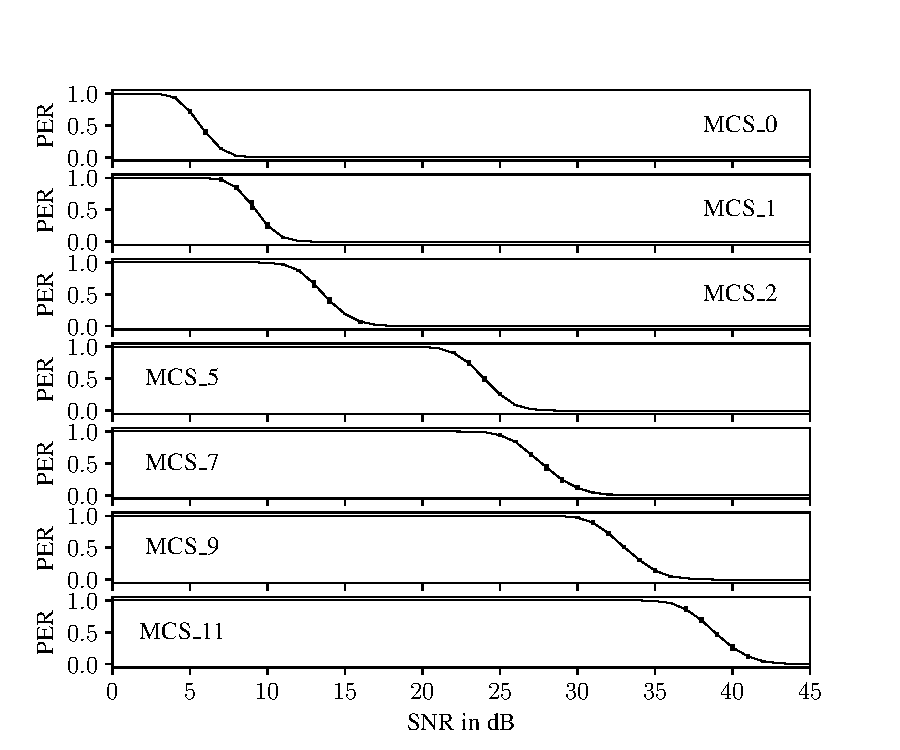
\includegraphics[width=0.95\textwidth]{figures/MCS_PER_to_SNR.pdf}
	\caption{Simulated PER in regards to SNR for chosen HE-MCS values for IEEE 802.11ax physical layer parameters
			of a GI of 3200 ns, a bandwidth of 20 MHz and 2 spatial streams.}
	\label{fig:PER_SNR_MCS}%
\end{figure}
\textcite{paul_characterizing_2011} conducted outdoor experiments to analyse the error rate and \ac{SNR} of different IEEE 802.11n \ac{MCS} for the
communication distances of \SI{300}{\meter}, \SI{800}{\meter} and \SI{1800}{\meter}. Their results show that \ac{SNR} decreases, when the transmissions range is longer.
Additionally, they experienced a higher error rate for higher.

The effect, that the \ac{PER} decreases, when the a lower \ac{MCS} or \ac{CR} is used, is the basis for the design of wifi rate managers.
A rate manager is a software component responsible to select physical layer parameters, such as \ac{MCS} or \ac{CR}, based on the current network conditions to
achieve the best possible throughput. Known rate managers of the linux kernel are the minstrel or the minstrel HT rate manager.

\subsubsection*{\acf{FEC}}
Another parameter that influences the \ac{PER} is the choice of the forward error correction (FEC) procedure. In order to
analyse the influence of the FEC procedure on the \ac{PER}, I simulated the \ac{PER} in regards to the \ac{SNR} for HE-MCS
\numrange{0}{9} and whether \ac{LDPC} or \ac{BCC} is enabled. For higher HE-MCS values \ac{BCC} can be used as \ac{LDPC} is compulsory, so no comparison of the \ac{FEC} procedures is possible.

The results are displayed in \autoref{fig:PER_SNR_LDPC}. The \ac{PER} decreases with higher \ac{SNR} for both \ac{FEC} procedures for all HE-MCS values as
expected. Using \ac{LDPC} instead of \ac{BCC}, a \ac{PER} of less than \SI{10}{\percent} can be achieved at \SI{2}{\decibel} higher \ac{SNR}
for all HE-MCS values. The effect increases to \SI{3}{\decibel} with higher HE-MCS values than HE-MCS \num{5}.
\begin{figure}[H]%
	\centering
	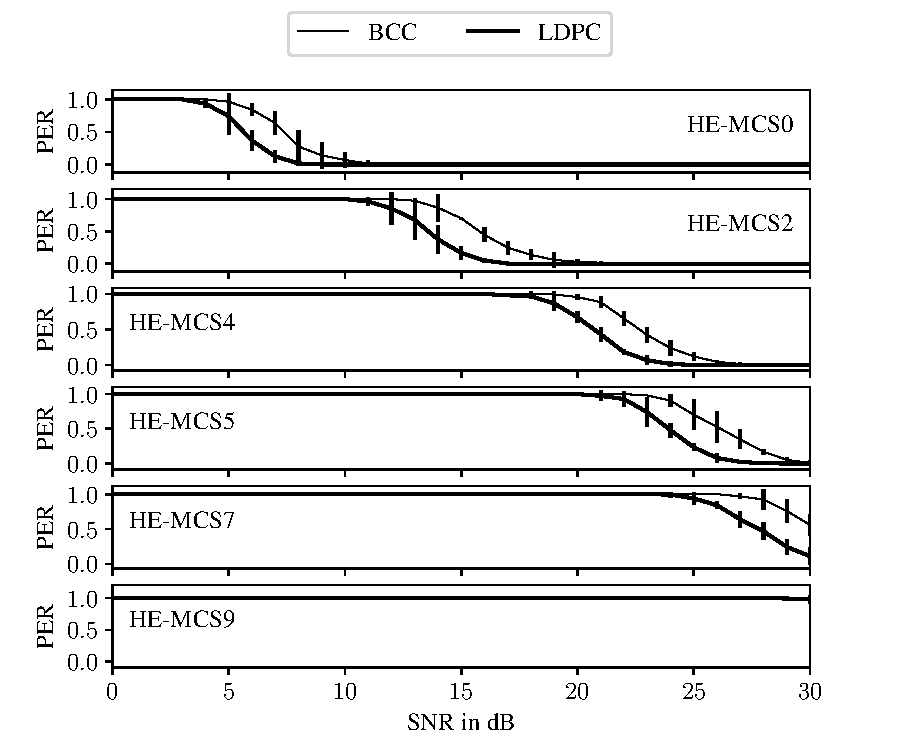
\includegraphics[width=0.95\textwidth]{figures/LDPC_PER_to_SNR.pdf}
	\caption{Simulated \ac{PER} in regards to \ac{SNR} for chosen HE-\ac{MCS} values and whether \ac{LDPC} or \ac{BCC} is enabled for IEEE 802.11ax physical layer parameters of a \ac{GI} of \SI{3200}{\nano\second}, a bandwidth of \SI{20}{\mega\hertz} and 2 spatial streams}%
	\label{fig:PER_SNR_LDPC}%
\end{figure}

\textcite{syafei_performance_2009} simulated the effect of the \ac{FEC} procedure on the \ac{PER} for IEEE 802.11n. They
had similar results and state, that using \ac{LDPC} instead of \ac{BCC}, a \ac{PER} of \SI{0.1}{\percent}  can be achieved at a
\SIrange{3.2}{6}{\decibel} higher \ac{SNR}.

According to \textcite{tran_asic_2014}, this effect is also present for IEEE 802.11ac. A \ac{PER} of \SI{0.1}{\percent} can be achieved at a
\SI{1.1}{\decibel} higher \ac{SNR} for using \ac{LDPC} instead of \ac{BCC} for 64 - \ac{QAM}. The effect increases to \SI{1.5}{\decibel} for 256 - \ac{QAM}.

\subsubsection*{\acf{GI}}

Robustness against intercarrier interference and intersymbol interference can be achieve by using a longer \ac{GI} \cite{pulimamidi_development_2007}. In order to analyse the impact of the \ac{GI} on the \ac{PER},
I simulated the \ac{PER} in regards to the \ac{SNR} for different HE-MCS values. The results for a \ac{GI} of \SI{3200}{\nano\second} and \SI{800}{\nano\second} are plotted in \autoref{fig:PER_SNR_GI}.
The \ac{PER} decreases with higher \ac{SNR} for all HE-MCS values as expected. Using a \ac{GI} of \SI{3200}{\nano\second} instead of \SI{800}{\nano\second} no significant difference of \ac{PER} in regards to the \ac{SNR} can be observed for HE-\ac{MCS} values lower than \num{5}.
Increasing the HE-\ac{MCS} value, the robustness of the \ac{MCS} sinks and the effect of the intercarrier interference and intersymbol interference increases.
As the maximum channel delay for the Tgax-F channel model is \SI{1050}{\nano\second}, the channel delay can be longer than the \ac{GI} of \SI{800}{\nano\second}. This
can result in intersymbol interference, which results in a higher \ac{PER} for higher HE-\ac{MCS} values.
For HE-\ac{MCS}\num{5}, a \ac{PER} of less than \SI{10}{\percent} can be achieved at \SI{1}{\decibel} lower \ac{SNR} for a \ac{GI} of \SI{3200}{\nano\second} instead of \SI{800}{\nano\second}. The effect increases
with higher HE-\ac{MCS} values.

\begin{figure}[H]%
	\centering
	
\includegraphics[width=0.95\textwidth]{figures/GI_PER_to_SNR.pdf}
	\caption{Simulated \ac{PER} in regards to \ac{SNR} for chosen HE-\ac{MCS} values and whether a \ac{GI} of \SI{800}{\nano\second} or \SI{3200}{\nano\second} is enabled for IEEE 802.11ax physical layer parameters of a bandwidth of \SI{20}{\mega\hertz} and 2 spatial streams}%
	\label{fig:PER_SNR_GI}%
\end{figure}
\textcite{patil_ieee_2020} conducted similar simulations for IEEE 802.11n.
They agree, that a longer \ac{GI} can increase the robustness against longer delay spreads as they are in the TGn-E and TGn-F channel models,
which are predecessors of the TGax-F channel model \cite{TGAXCHANNEL}.
\begin{comment}
	cite others seane old?? Evelt Van Duc Nguyen, 2016

\end{comment}



\subsubsection*{\acf{DCM}}
Next, I simulated the \ac{PER} in regards to the \ac{SNR}  and whether \ac{DCM} is enabled for the specfied HE-\ac{MCS} values. Dabei habe ich für die SImulation die möglichen
HE-MCS \num{0},\num{1},\num{3} and \num{4} aus dem IEEE 802.11ax Standard verwendet.

The results indicate, that using \ac{DCM} can achieve the same \ac{PER} at lower \ac{SNR} values compared to not using \ac{DCM}. A \ac{PER} of less than \SI{10}{\percent} can be achieved at
a \SI{2}{\decibel} lower \ac{SNR} when using \ac{DCM}.
The effect increases to \SI{4}{\decibel} for higher HE-\ac{MCS}\num{4}.
The results are plotted in \autoref{fig:PER_SNR_DCM}.
\begin{figure}[H]%
	\centering
	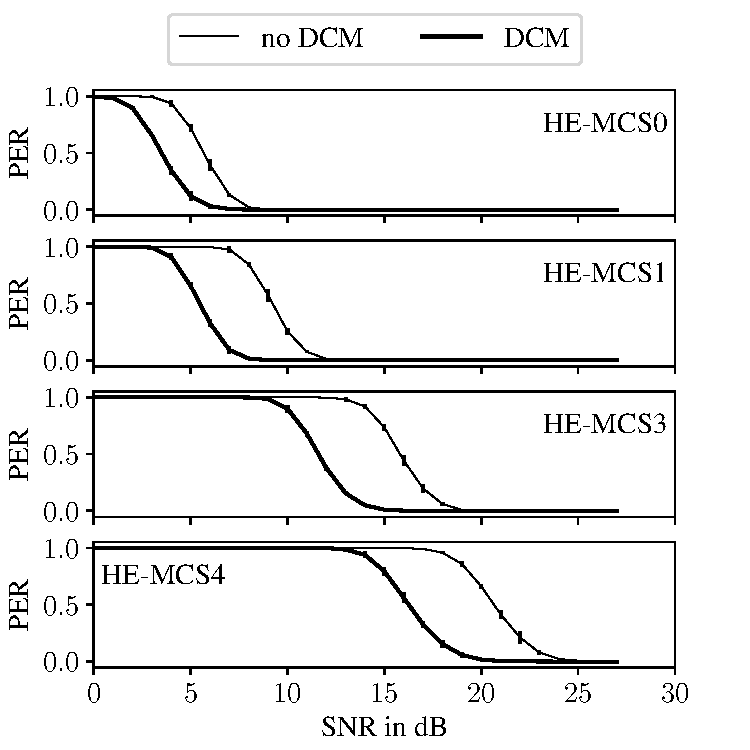
\includegraphics[width=0.95\textwidth]{figures/DCM_PER_to_SNR.pdf}
	\caption{Simulated \ac{PER} in regards to \ac{SNR} for chosen HE-\ac{MCS} values and whether \ac{DCM} is enabled for IEEE 802.11ax physical layer parameters of a \ac{GI} of \SI{3200}{\nano\second}, a \ac{BW} of \SI{20}{\mega\hertz} and 2 spatial streams}%
	\label{fig:PER_SNR_DCM}%
\end{figure}


\Textcite{ryu_ber_2010} and \textcite{park_ber_2006} conducted a similar simulation, where they analyse the bit error rate in
regards to the normalized \ac{SNR} and whether \ac{DCM} was enabled for rayleigh fading channels. Both authers wraped two
Quadrature \ac{PSK} modulated symbols into one 16-\ac{QAM} symbol. As Quadrature \ac{PSK} modulates \SI{2}{\bit} per symbol, the infomation
of two Quadrature \ac{PSK} modulated symbols can be
transmitted in one 16-\ac{QAM} symbol, which encodes \SI{4}{\bit}. The authors transmit the 16-\ac{QAM} symbols and a redundant copy
of the 16-\ac{QAM} symbols via orthogonal subcarriers. At the receiver the authors combine the copies and retrieve the transmitted
information using the Maximum likelyhood criterion. The results of the author show that a better bite error rate can be achieved while applying
\ac{DCM} than sending the information via two Quadrature \ac{PSK} or 16-\ac{QAM} modulated symbols without \ac{DCM}.
\cite{khorov_ieee_2015} DCM 2db gain


\subsubsection*{\acf{ER}}
For a HE-MCS \num{0} and \num{1} the \ac{ER} range mode can be applied additional to \ac{DCM}, when one spatial stream is used \cite{noauthor_ieee_2021}.
In order to analyse the impact of the \ac{ER} mode, I set the physical layer parameters to a \ac{GI} of
\SI{3200}{\nano\second}, a \ac{BW} of \SI{20}{\mega\hertz} and one spatial streams. For He-MCS \num{0}, \num{1} and \num{3} I run simulations, where I enabled the
\ac{ER} mode and compared the \ac{PER} to the \ac{PER} of the same HE-MCS values without \ac{ER} mode.

The results in \autoref{fig:PER_SNR_ER} indicate , that the \ac{PER} is influenced by the \ac{ER} mode.
The difference in \ac{SNR} with \ac{ER} mode to without \ac{ER} mode, where a \ac{PER}
of \SI{10}{\percent} is achieved, is \SIrange{1}{2}{\decibel}.
\begin{comment}
	{'mcs0_1_er.csv': [7.0, 6.0, 3.0], 'mcs1_2_er.csv': [11.0, 10.0, 6.0], 'mcs2_3_er.csv': [16.0, 14.0]}
\end{comment}
\begin{figure}%
	\centering
	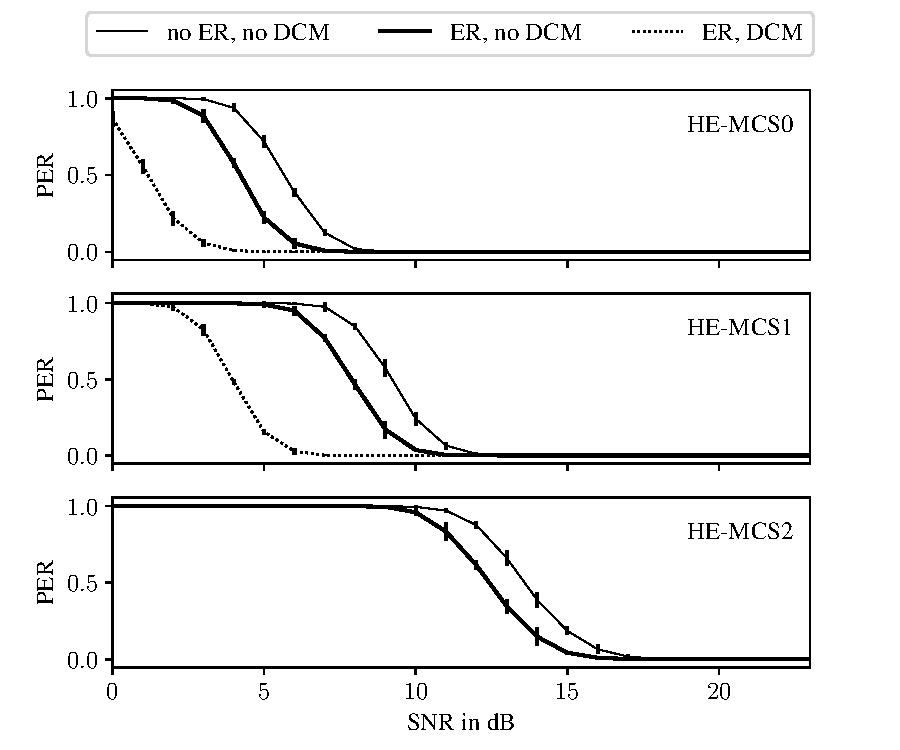
\includegraphics[width=0.95\textwidth]{figures/ER_PER_to_SNR.pdf}
	\caption{Simulated \ac{PER} in regards to \ac{SNR} for chosen HE-\ac{MCS} values and whether Extended Range or \ac{DCM}
	is enabled for IEEE 802.11ax physical layer parameters of a \ac{GI} of \SI{3200}{\nano\second}, a \ac{BW} of \SI{20}{\mega\hertz} and 2 spatial streams}
	\label{fig:PER_SNR_ER}%
\end{figure}

Additionally, I simulated the impact of applying the \ac{ER} mode and \ac{DCM} for the allowed HE-MCS values \num{0} and \num{1}.
Applying \ac{DCM} additionally makes the transmission more robust. As it is displayed in \autoref{fig:PER_SNR_ER_DCM},
a \ac{PER} of less than \SI{10}{\percent} can be achieved at a \SIrange{4}{5}{\decibel} lower \ac{SNR} when using \ac{DCM} and \ac{ER} mode together instead
of using \ac{ER} mode alone.

\textcite{jacob_system-level_2020} conducted a simulation, where they analysed the effect of \ac{DCM} and \ac{ER} on the \ac{PER} for
IEEE 802.11bd in vehicular environments to the transmission range. The authors found out, that the using \ac{DCM} and \ac{ER} can
increase the transmission range for \ac{LoS} by \SI{65}{\percent} for a \ac{PER} greater than \num{0.1}. After additional analysis with higher
vehicle densities, the authors remark, that using \ac{DCM} and the \ac{ER} mode cause channel congestion in CSMA/CA based
networks with low bandwidths. The authors conclude, that the \ac{ER} mode and \ac{DCM} should be used for long range transmissions, where
the physical layer parameters can extend the transmission range significantly.

A similar simulation was conducted by \textcite{triwinarko_phy_2021}. The researchers state, that using \ac{DCM} and the
\ac{ER} mode results in better \ac{PER} performance at lower \ac{SNR} values in \ac{LoS} and non \ac{LoS} scenarios.

\subsubsection*{\acf{STBC}}
As aforementioned, additional robustness can be achieved by applying \ac{STBC}. In order to analyse the impact of \ac{STBC} on the \ac{PER} in regards to the \ac{SNR},
I run the simulation for the HE-MCS values \numrange{0}{11} with and without \ac{STBC}.

The results in \autoref{fig:PER_SNR_STBC} indicate, that the \ac{PER} is influenced
by the \ac{STBC} mode. A \ac{PER} of less than \SI{10}{\percent} is possible at a \SIrange{2}{10}{\decibel} lower \ac{SNR} when using \ac{STBC} additionally.
The impact of \ac{STBC} on the \ac{PER} grows from \SI{2}{\decibel} for HE-MCS\num{0} to \SI{10}{\decibel} for HE-MCS\num{11}.
\begin{comment}
	{'mcs0_stbc.csv': [7.0, 5.0], 'mcs2_stbc.csv': [16.0, 8.0], 'mcs9_stbc.csv': [36.0, 26.0],
		'mcs7_stbc.csv': [30.0, 20.0], 'mcs5_stbc.csv': [26.0, 18.0], 'mcs1_stbc.csv': [11.0, 6.0], 'mcs11_stbc.csv': [41.0, 31.0]}
\end{comment}

\begin{figure}%
	\centering
	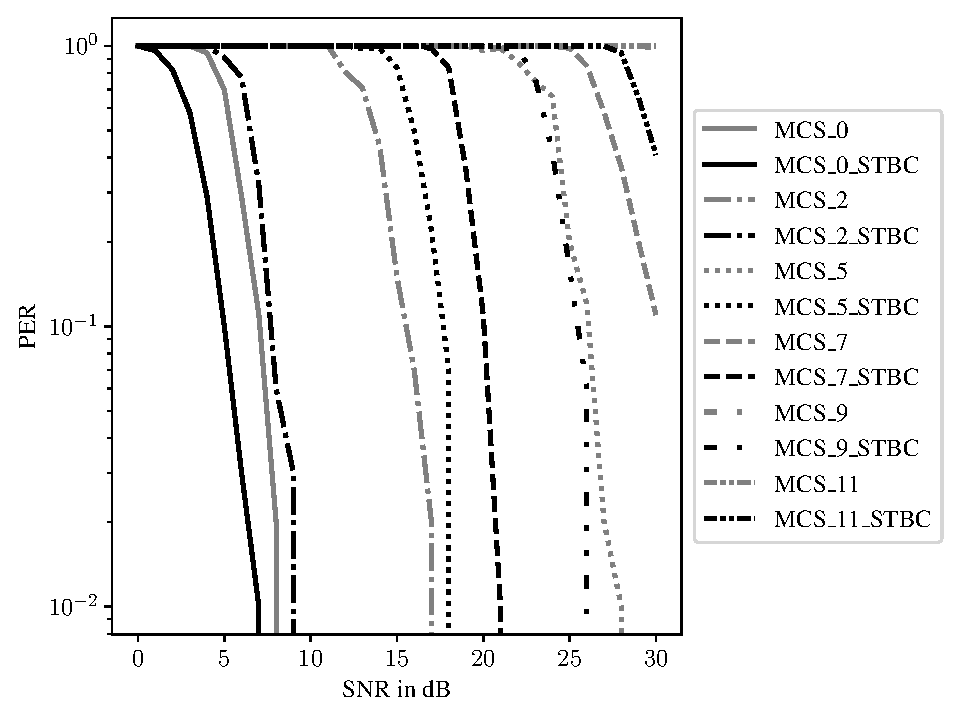
\includegraphics[width=0.95\textwidth]{figures/STBC_PER_to_SNR.pdf}
	\caption{Simulated \ac{PER} in regards to \ac{SNR} for chosen HE-\ac{MCS} values and whether \ac{STBC} is enabled for IEEE 802.11ax physical layer parameters of a \ac{GI} of \SI{3200}{\nano\second}, a \ac{BW} of \SI{20}{\mega\hertz} and 2 spatial streams}%
	\label{fig:PER_SNR_STBC}%
\end{figure}
\textcite{stamoulis_impact_2003} analysed the impact of \ac{STBC} on the bit error rate for IEEE 802.11a in regards to the \ac{SNR}. Their simulation was based
on a HiperLAN/2 channel with \num{2} antennas. They used HiperLAN/2, because it has a similar physical layer as IEEE 802.11a.
The authors found out, that applying \ac{STBC} results in a lower bit error rate for a given \ac{SNR} value. The authors conclude, that \ac{STBC} can be used to
\textcite{santumon_space-time_2012} and \textcite{tarokh_space-time_1999} conducted simulations, where they analysed the effect of \ac{STBC} on the bit error rate for
wireless communication systems. In general, the authors found out, that \ac{STBC} can be used to increase the bit error rate for a given \ac{SNR} value for different
\ac{MCS} values. Additionally, the authors remark, that the impact of \ac{STBC} on the bit error rate grows with the number of antennas.
However, the number of antennas is limited to \num{2} for IEEE 802.11ax \cite{noauthor_ieee_2021}.

The robustness analysis results indicate, which \ac{PER} decreases can be achieved by applying the different phsyical layer parameters.
The intensity of the impact varies depending on the environment and the actual communication channel.

I conducted the same simulations for the frequency band of \SI{2.4}{\giga\hertz}. Using the same physical layer parameters in
the \SI{2.4}{\giga\hertz} band achieve a similar \ac{PER} in regards to the \ac{SNR} and chosen physical layer parameters
as in the \SI{5}{\giga\hertz} band.

But how does the effect of the frequency bands on the \ac{PER} in regards to the \ac{SNR} differ?
Taking the Friis transmission model \cite{shaw_radiometry_2013} into account, the \ac{RSS} for omnidirectional antennas can be calculated in regard to the distance $d$,
receiving antenna gain $G_{R}$, transmitting antenna gain $G_{T}$ and transmission power $P_{T}$  as follows:
\begin{equation}
	RSS = P_{T} * G_{T} * G_{R} * \frac{\lambda^2}{(4 * \pi * d)^2}.
\end{equation}
When $\lambda$ is replaced and  $P_{T}$,  $G_{T}$,  and $G_{R}$ are set to \num{1} the following equation can be derived:
\begin{equation}
	RSS = \frac{c^2}{(f* 4 * \pi * d)^2},
\end{equation}
where $c$ is the speed of light and $f$ is the frequency of the transmission.
Converting the equation to $d$ it results in the following equation:
\begin{equation}
	d = \frac{c}{(4 * \pi * f * \sqrt {RSSI})}.
\end{equation}
The equation shows, that a lower frequency results in a higher \ac{RSS} for a given distance.
This means, that the \SI{2.4}{\giga\hertz} band can achieve a higher \ac{SNR} for a given distance and noise floor
compared to the \SI{5}{\giga\hertz} band.
The simulation results can now be used to derive the following conclusion,
that a lower \ac{PER} for the \SI{2.4}{\giga\hertz} band can be accomplished
for a given set of physical layer parameters, distance and noise floor.


\todo{What should be chosen?}